\appendix

\chapter{Appendix}
Appendix content goes here.

\section{Mockups}
After the second meeting with the customer, the group had a sketch that was to be used as a starting point for the mock-up application.
\pagebreak
\begin{figure}[here]
\setlength\fboxsep{0pt}
\setlength\fboxrule{1pt}
\fbox{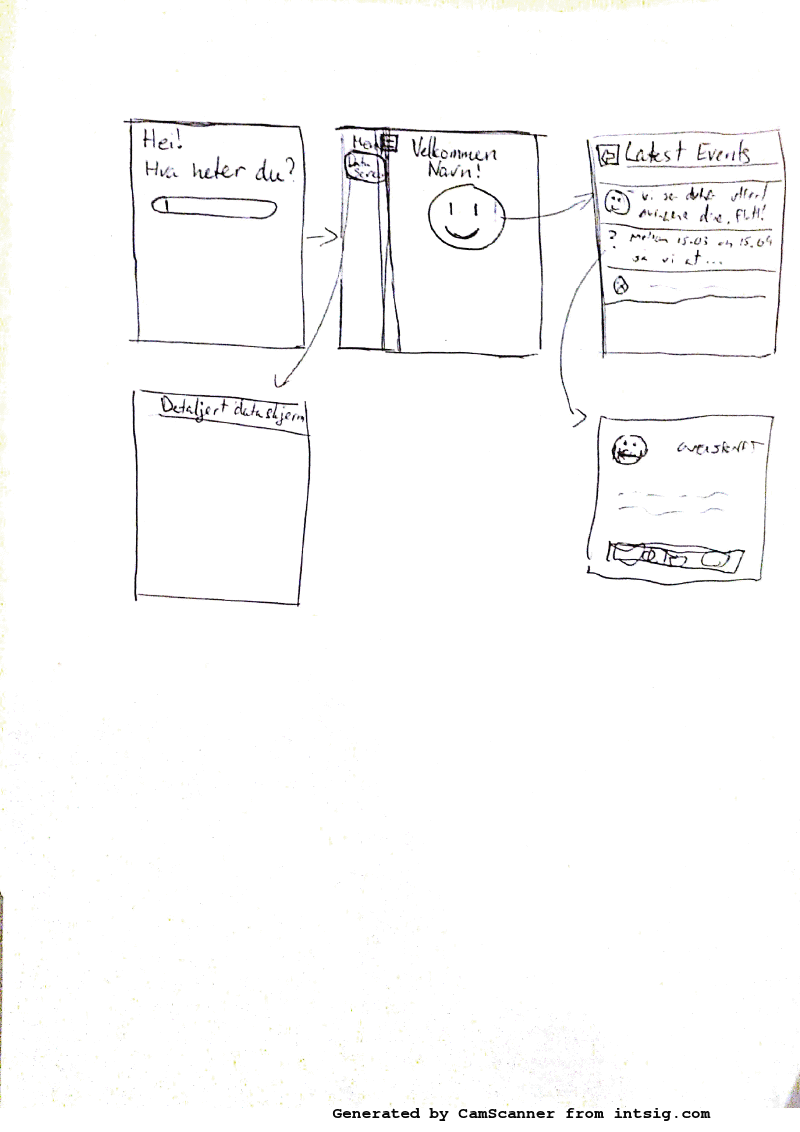
\includegraphics[trim = 20mm 180mm 0mm 20mm, clip, width=\linewidth]{Res/mockupV2}}
\caption{A mockup of the program flow, text is just scribbling}
\label{fig:mockupV2}
\end{figure}


\section{Reports}

\begin{figure}
\caption{Short summary of work done sorted by sprint}
\begin{tabular}{|c|c|p{7cm}|}
\hline
Sprint nr. & Date & Summary\\
\hline
Sprint 1: & 03.02.13 - 08.02.13 & Developing user stories and paper prototypes of the GUI.\\ 
\hline
Sprint 2: & 08.02.13 - 15.02.13 & Developing a mock-up application demonstrating the GUI.\\
\hline
Sprint 3: & 15.02.13 - 22.02.13 & Improving UI and functionality for the prototype, researching medicinal factors. \\
\hline
Sprint 4: & 22.02.13 - 01.03.13 & Improving secondary functionality for the prototype (settings, statistics, relatives screens),researching contentproviders and alternative solutions. \\
\hline

\end{tabular} 
\label{tab:sprintList}

\end{figure}